\documentclass[a4paper,11pt]{article}

%%%%%%%%%%%%%%%%%%%%%%%%%%%%%%%%%%%%%%%%%%%%%%%%%%%%%%%%%%%%

% Global structure parameters
\usepackage{fullpage}%

\usepackage[francais]{babel}%

\usepackage[utf8]{inputenc}%
\usepackage[T1]{fontenc}%

% Font selection: http://www.tug.dk/FontCatalogue/newpx/
\usepackage{newpxtext}%
\usepackage{newpxmath}%

% Macro packages
\usepackage{url}%
\usepackage{graphicx}%
\usepackage{listings}%

% Parameters for listings

\usepackage[table]{xcolor}

% Fine tuning
\setlength{\parskip}{0.2\baselineskip plus 0.2\baselineskip}%

%%%%%%%%%%%%%%%%%%%%%%%%%%%%%%%%%%%%%%%%%%%%%%%%%%%%%%%%%%%%

\begin{document}

\title{Rapport du projet 7 couleurs}

\author{Le Dilavrec Quentin et Clément Legrand Lixon}

\date{15 octobre 2017}

\maketitle

\begin{abstract}
Le jeu des 7 couleurs est un jeu vidéo de stratégie, que nous avons réimplémenté en C. Ce rapport a pour but de répondre 
clairement et de façon détaillée à chacune des questions  que nous avons
traitées et présentes dans le sujet du projet.
\end{abstract}

%%%%%%%%%%%%%%%%%%%%%%%%%%%%%%%%%%%%%%%%%%%%%%%%%%%%%%%%%

\section{Introduction}
Le jeu des 7 couleurs aussi appelé Filler dans sa version anglophone est 
un jeu vidéo de stratégie/puzzle créé par Dmitry Pashkov et pour la première 
fois publié par la société Gamos pour MS-DOS en 1990! De par son gameplay 
très simple, peu d'intéractions avec l'utilisateur tant du point de vue des commandes 
jouées par le(s) utilisateur(s) que par l'affichage facilement faisable dans le shell. 
Le jeu est donc parfaitement adapté aux programmeurs débutants en C. Le sujet est 
pésenté sous la forme de questions, chacune portant sur une partie particulière du jeu, 
de l'affichage à l'interaction avec l'utilisateur pour finir avec les IA.

%%%%%%%%%%%%%%%%%%%%%%%%%%%%%%%%%%%%%%%%%%%%%%%%%%%%%%%%%

\section{L'affichage}

Dans cette première partie, nous nous sommes intéressés à l'affichage
du monde des 7 couleurs, ainsi que sa mise à jour après un coup d'un des
joueurs.

\subsection{Initialisation du plateau de jeu}
\emph{Réponse de Q1}

Pour permettre l'initialisation du plateau de jeu, il faut choisir de manière aléatoire l'une des 7 couleurs disponibles, représentées par la suite par une lettre (A, B, C, ..., G). Il suffit alors de tirer un entier aléatoire entre 1 et 7 puis de le remplacer par la lettre correspondante dans le plateu de jeu. 

Pour cela nous avions dans un premier temps  utilisé la fonction rand() disponible en C, qui renvoie un entier, puis on calculait le reste de sa division par 7 pour obtenir un entier entre 0 et 6. 

Toutefois pour plus de lisibilié et la modularité on utilise 
\begin{lstlisting}[language=C, caption=parameters.h]
...
#define COLORS_NUMBER 7
...
\end{lstlisting}

\begin{lstlisting}[language=C, caption=board.h]
...
#define RANDOM_COLOR (1 + (int)(rand() % COLORS_NUMBER))
...
\end{lstlisting}

Puis on parcourt le tableau avec deux boucles "for" imbriquées et on attribue pour chaque cellule une valeur aléatoire avec RANDOM\_COLOR

Ensuite on rempli les cases (29,0) et (0,29) pour qu'elles contiennent respectivement les symboles des joueurs 1 et 2.

A l'issue de cette initialisation, nous pouvons nous intéresser au déroulement du jeu en lui-même.

\subsection{Mise à jour du plateau}
\emph{Réponse de Q2}

Pour pouvoir (enfin) jouer au jeu, il faut que le plateau se mette à jour automatiquement une fois que l'un des joueurs a joué une lettre. Pour ce faire on parcourt le monde linéairement jusqu'à tomber sur une lettre à la fois choisie et voisine d'un symbole joueur. Dans ce cas on remplace la lettre trouvée par un symbole joueur, on poursuit jusqu'à avoir fait tout le plateau et, s'il y a eu une modification, on recommence le parcours du monde du début, de cette façon on est sûr de n'oublier aucune lettre lors de la mise à jour, et l'algorithme se termine bien puisqu'il n'y a qu'un nombre fini de cases dans le plateau de jeu. Pour vérifier que cette fonction affiche le résultat voulu, il suffit de la tester sur un plateau, de rentrer une lettre et de vérifier qu'il ne reste plus de lettres choisies adjacentes à un symbole joueur. 

Le pire cas est obtenu lorsque le joueur se trouve dans la cellule parcouru en dernier et que le plateau ne contient qu'une seule lettre et qu'elle est choisie par un joueur. On peut illustrer ce cas avec le schéma suivant, la première image correspond à la situation initiale, chacune des images suivantes montre le tableau à la fin de la double boucle "for", ce qui correspond à l'intégration de tous les voisins adjacents qu'il est possible d'avoir. Dans ce cas il y a 31 parcours du monde (autant qu'il y a de diagonales).

\begin{figure}[!h]
\begin{center}
\begin{tabular}{ | l | c | r | }
	\hline
	A & A & A \\ 
	\hline
	A & A & A \\ 
	\hline
	A & A & \cellcolor{blue!25}v \\
	\hline
\end{tabular}
\hspace{1cm}
{\Huge
\begin{math}
\Rightarrow
\end{math}}
\hspace{1cm}
\begin{tabular}{ | l | c | r | }
	\hline
	A & A & A \\ 
	\hline
	A & A & \cellcolor{blue!25}v \\ 
	\hline
	A & \cellcolor{blue!25}v & \cellcolor{blue!25}v \\
	\hline
\end{tabular}
\hspace{1cm}
{\Huge
\begin{math}
\Rightarrow
\end{math}}
\hspace{1cm}
\begin{tabular}{ | l | c | r | }
	\hline
	A & A & \cellcolor{blue!25}v \\ 
	
	\hline
	A & \cellcolor{blue!25}v & \cellcolor{blue!25}v \\ 
	
	\hline
	
	\cellcolor{blue!25}v & \cellcolor{blue!25}v & \cellcolor{blue!25}v \\
	\hline
\end{tabular}
\end{center}
\caption{Evolution du plateau dans le pire cas avec modify}
\end{figure}

\subsection{Amélioration du parcours du monde}
\emph{Réponse Q3 (bonus)}

La méthode de mise à jour précédente est particulièrement inefficace dans son
pire cas, et on peut l'améliorer de la manière suivante : on parcourt le monde
jusqu'à trouver une lettre choisie voisine d'un symbole joueur, on place les coordonnées de
cette lettre dans une pile. On garde en mémoire ces coordonnées, puis on dépile et
on regarde si cette lettre est entourée de lettres semblables (dans le sens horaire, 
en partant du nord par exemple), on empile les coordonnées des lettres voisines semblables,
on remplace la lettre sur laquelle on était par un symbole joueur,
et tant que la pile n'est pas vide on procède de la même façon. Dès que la pile est vide
on retourne à la première case qui s'est empilée(celle qu'on a gardée en mémoire au début), puis on continue le parcours 
du plateau, en faisant la même chose dès qu'on tombe sur une nouvelle lettre choisie
qui est voisine d'un symbole joueur. De cette façon on ne parcourt plus que 2 fois
seulement le monde dans le pire cas. Toutefois nous n'avons pas eu le temps
d'implémenter l'algorithme en C.

Le schéma suivant indique ce qu'il se passe :
on tombe d'abord sur la lettre A (en rouge), c'est cette case dont on
se souviendra par la suite pour continuer le parcours (elle passe au vert
après avoir été changée en symbole), on regarde ensuite ses voisines, il y aussi
une lettre A (on la met en rouge car elle va dans la pile), et continue ainsi de 
suite (mais on ne met plus de cases en vert) jusqu'à ce que la pile soit vide, puis
on continue le parcours depuis la case verte. Ensuite si on trouve une nouvelle
lettre A voisine de v elle va dans la pile et on recommence...


\begin{figure}[!h]
\begin{center}
\begin{tabular}{ | l | c | r | }
	\hline
	A & A & A \\ 
	\hline
	B & B & A \\ 
	\hline
	B & A & \cellcolor{blue!25}v \\
	\hline
\end{tabular}
\hspace{0.1cm}
{\Huge
\begin{math}
\Rightarrow
\end{math}}
\hspace{0.1cm}
\begin{tabular}{ | l | c | r | }
	\hline
	A & A & A \\ 
	\hline
	B & B & \cellcolor{red!25}A \\ 
	\hline
	B & A & \cellcolor{blue!25}v \\
	\hline
\end{tabular}
\hspace{0.1cm}
{\Huge
\begin{math}
\Rightarrow
\end{math}}
\hspace{0.1cm}
\begin{tabular}{ | l | c | r | }
	A & A &\cellcolor{red!25}A \\ 
	\hline
	B & B & \cellcolor{green!25}v \\ 
	\hline
	B & A & \cellcolor{blue!25}v \\
	\hline
\end{tabular}
\hspace{0.1cm}
{\Huge
\begin{math}
\Rightarrow
\end{math}}
\hspace{0.1cm}
\begin{tabular}{ | l | c | r | }
	\cellcolor{blue!25}v & \cellcolor{blue!25}v &\cellcolor{blue!25}v \\ 
	\hline
	B & B & \cellcolor{blue!25}v \\ 
	\hline
	B & \cellcolor{red!25}A & \cellcolor{blue!25}v \\
	\hline
\end{tabular}
\end{center}
\caption{Evolution du plateau avec la pile}

\end{figure}
%%%%%%%%%%%%%%%%%%%%%%%%%%%%%%%%%%%%%%%%%%%%%%%%%%%%%%%%%


\section{Les interactions avec l'utilisateur}

A présent nous allons développer une implémentation Humain/Humain, pour 
pouvoir jouer au jeu 7colors à deux.

\subsection{De quoi jouer faire un duel entre utilisateurs}
\emph{Réponse de Q4}

Pour que deux joueurs humains puissent s'affronter dans ce jeu, il faut d'abord s'assurer que chaque joueur puisse jouer l'un après l'autre. Il suffit pour cela  de choisir de manière arbitraire quel joueur commencera la partie (ici J1), puis on incrémente notre variable de un à chaque fois qu'un joueur à joué (on repasse à J1 quand on dépasse le nombre de joueurs). Il suffit ensuite de demander au joueur une lettre à remplacer pour agrandir sa zone, puis de mettre à jour le plateau de jeu.

Toutefois il peut aussi arriver que l'un des deux joueurs tape (de manière tout à fait malencontreuse) un caractère différent de l'une des lettres attendues  (c'est-à-dire une lettre autre que majuscule (ou minuscule) entre A et G), et dans ce cas on doit renvoyer un message d'erreur adapté pour que le joueur puisse corriger.
Comme par exemple on peut obtenir le message d'erreur suivant si on tape 'n' :

\begin{figure}[!h]
\begin{center}
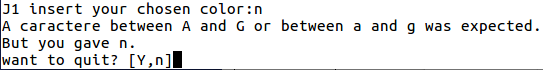
\includegraphics[width=0.8\textwidth]{erreur.png}
\caption{Message d'erreur si l'utilisateur se trompe}
\end{center}
\end{figure}
Comme aucune condition de victoire n'a été définie, la partie entre les deux joueurs est sans fin... Il est temps d'y remédier !  


\subsection{Conditions de victoire}
\emph{Réponse de Q5}

Une première idée serait d'arrêter la partie seulement lorsque le monde est
divisée en deux zones, puis de comparer le nombre de cases de chacun des joueurs.
Toutefois, dès que l'un des deux joueurs possède au moins 50\% du plateau, l'autre joueur
ne pourra plus gagner : c'est notre condition de victoire. 

Ainsi la partie s'arrête dès que l'un des deux joueurs possède au moins 50\% du plateau.
On verifie donc à chaque tour que le pourcentage de cases possédées par chaque joueur ne dépasse pas $BOARD\_SIZE^2/PLAYERS\_NUMBER$, et si c'est le cas la partie s'arrête. Bien sûr pour ne pas faire le parcours de tout le plateau à chaque tour on stocke le nombre de cellules possédées par chaque joueur (c'est "modify" qui le maintient à jour).


%%%%%%%%%%%%%%%%%%%%%%%%%%%%%%%%%%%%%%%%%%%%%%%%%%%%%%%%%

\section{Les intelligences artificielles aléatoires}

C'est bien de pouvoir jouer à deux, mais on n'a pas toujours d'amis sous la
main, et pour pallier à ce problème nous allons nous intéresser à présent 
à l'implémentation de certaines Intelligences artificielles.

\subsection{Jouer totalement aléatoirement}
\emph{Réponse de Q6}

La première IA à programmer doit choisir aléatoirement une couleur parmi 
les 7 du jeu, lorsque c'est son tour. Pour ce faire il suffit de reprendre 
l'implémentation pour un joueur humain, sauf qu'au lieu de rentrer une couleur
soi-même, elle est choisie de manière aléatoire (comme quand on rempli le tableau
pour la première fois (cf Question 1)). Le plateau est ensuite mis à jour 
et affiché. On demande également à ce que la couleur choisie soit affichée.

Le fonctionnement de cette IA est illustré à travers les images suivantes (c'est J1):

\begin{figure}[!h]
\begin{center}
\includegraphics[width=0.2\textwidth]{a1(init).png}
{\Huge
\begin{math}
\Rightarrow
\end{math}}
\includegraphics[width=0.2\textwidth]{a1(1).png}
{\Huge
\begin{math}
\Rightarrow
\end{math}}
\includegraphics[width=0.2\textwidth]{a1(last).png}
\caption{Intelligence artificielle aléatoire (au début, après un coup, et au dernier tour)}
\end{center}
\end{figure}

On peut observer, après plusieurs parties, que cette IA est particulièrement 
inefficace, on va donc s'intéresser à une IA aléatoire plus efficace.


\subsection{Jouer aléatoirement plus intelligemment}
\emph{Réponse de Q7}

Cette IA, a pour objectif d'être plus efficace que l'IA précédente. On va donc
s'intéresser cette fois à une IA qui choisi une couleur aléatoirment mais 
seulement parmi les couleurs qui peuvent agrandir sa zone. 

Pour connaître les couleurs adjacentes à l'IA, on initialise un tableau de
booléens B avec des "false", puis on parcourt le plateau jusqu'à tomber sur une lettre qui possède 
un voisin correspondant au symbole de l'IA, on transforme ensuite la lettre 
en un chiffre n puis le n-ième élément de B prend la valeur "true", puis on continue
le parcours du plateau. A la fin on obtient un tableau B de booléens dont les indices correspondent aux couleurs, ce qui permet de connaître
les couleurs adjacentes à l'IA. Il suffit ensuite de mettre les couleurs de valeur "true" dans B dans un tableau C. Ensuite on choisit un entier au hasard compris entre 0 et l'indice où on s'est arrêté de mettre des couleurs dans C. On renvoie alors la couleur lue.

Le fonctionnement de cette IA est illustré à travers les images suivantes (c'est J1):

\begin{figure}[!h]
\begin{center}
\includegraphics[width=0.2\textwidth]{a2(init).png}
{\Huge
\begin{math}
\Rightarrow
\end{math}}
\includegraphics[width=0.2\textwidth]{a2(1).png}
{\Huge
\begin{math}
\Rightarrow
\end{math}}
\includegraphics[width=0.2\textwidth]{a2(last).png}
\caption{Intelligence artificielle aléatoire améliorée (au début, après un coup, et au dernier tour)}
\end{center}
\end{figure}
Cette IA est nettement plus efficace que la précédente mais peut-on faire mieux ?

%%%%%%%%%%%%%%%%%%%%%%%%%%%%%%%%%%%%%%%%%%%%%%%%%%%%%%%%%

\section{L' intelligence artificielle gloutonne}

La partie précédente nous a permis de développer des intelligences artificielles
basées sur l'aléatoire, mais l'aléatoire a souvent des limites. Une idée naïve pour
qu'une IA gagne serait qu'à chaque tour elle essaie de récupérer le maximum de cases
autour d'elle. L'objectif de cette partie est donc d'implémenter cette IA, qualifiée 
de gloutonne, puis de la comparer à l'IA aléatoire implémentée précédemment.


\subsection{Maximisation du gain en cases immédiate}
\emph{Réponse de Q8}

Pour implémenter cette nouvelle IA, on construit une copie vierge du plateau de jeu (où l'on ajoute les cases du joueur actuel),
ainsi qu'un tableau d'entiers T, dont chaque case contiendra le nombre de cases que l'IA peut
avoir en jouant la lettre associée. 

On commence par parcourir le plateau de jeu, lorsqu'on tombe sur une lettre voisine
d'un symbole joueur, ou voisine de la même lettre dans le plateau copie, on place cette
lettre dans le plateau copie à la même place que dans le vrai plateau, on incrémente
la i-ème case de T de 1 (avec i le nombre associé à la lettre trouvée) et on 
recommence le parcours du plateau du début tant que l'on a modifié une case durant cette boucle. A la fin, T contient le nombre de cases
que l'IA pourra récupérer en jouant une lettre, il suffit alors de récupérer l'indice
du maximum de T, puis l'IA jouera la couleur associée à cet indice. 

Le fonctionnement de cette IA est illustré à travers les images suivantes (c'est J1):

\begin{figure}[!h]
\begin{center}
\includegraphics[width=0.2\textwidth]{g(init).png}
{\Huge
\begin{math}
\Rightarrow
\end{math}}
\includegraphics[width=0.2\textwidth]{g(2).png}
{\Huge
\begin{math}
\Rightarrow
\end{math}}
\includegraphics[width=0.2\textwidth]{g(last).png}
\caption{Intelligence artificielle gloutonne (au début, après deux coups, et au dernier tour)}
\end{center}
\end{figure}

Nous obtenons ainsi une IA qui cherche à maximiser son nombre de cases à chaque tour,
essayons maintenant de faire jouer notre IA aléatoire améliorée et cette IA, pour
savoir laquelle est la meilleure.

\subsection{Aléatoire contre Glouton}
\emph{Réponse de Q9}

Pour ne pas désavantager une IA par rapport au l'autre, il faut qu'il y ait une répartition homogène des lettres dans le plateau (on ne doit pas avoir une lettre surreprésentée car sinon Glouton pourrait facilement être avantagée en tombant sur ce groupe de lettres, alors que pour avantager l'IA aléatoire, il faudrait qu'à chaque tour cette IA n'ait qu'un seul choix possible). Ainsi pour des plateaux totalement aléatoires de 30X30, aucune des deux IA ne peut réellement être avantagée. 

L'IA aléatoire améliorée ne gagne jamais contre le glouton, ce qui ne fait pas des valeurs très intéressantes à étudier.

\subsection{Championnat}
\emph{Réponse de Q10}

En faisant en championnat de 100 parties on remarque que c'est toujours Glouton qui gagne. Ce qui est peu surprenant en fait puisque l'IA aléatoire n'a pas vraiment de stratégie gagnante. 

Cela peut s'expliquer en terme de probabilités, en effet considérons le cas où il n'existe qu'un seul chemin pour accéder à la victoire (un tel chemin existe car le glouton a un chemin entièrement déterminé et il gagne à chaque fois). Dès lors il faut qu'à chaque tour l'IA choisisse aléatoirement parmi au plus 6 couleurs (on vient de jouer une couleur) le bon chemin. Pour un tour donné la probabilité que l'IA choisisse une lettre du chemin gagnant est d'au moins $1/6$. De plus on peut remarquer que l'algorithme glouton gagne en environ 40 tours, il faudrait donc que l'IA choisisse 40 fois d'affilée la bonne lettre ce qui laisse une probabilité de victoire d'environ $(1/6)^{40}$ (en réalité sa probabilité de victoire est plus élevée, car il n'y a pas qu'un seul chemin gagnant, et l'IA ne doit pas toujours choisir entre 6 couleurs).

\section{Conclusion}

A travers ce projet nous avons pu implémenter le jeu 7colors et diverses IA
pour jouer avec nous. Ca n'a pas toujours été facile d'implémenter de manière
efficace les IA, mais le tout était intéressant pour un premier projet en C, ce qui
a notamment permis de mettre en pratique tout ce que nous avions vu en cours et d'approfondir certains points plus techniques (pointeurs notamment), d'autant plus que l'objectif est aussi de produire un code propre et lisible pour que d'autres personnes puissent le lire. 
Finalement c'était un projet amusant et assez bien adapté aux débutants en C mais plus de code pour le squelette aurais peut être permis de s'intéréser plus rapidement à des points intéréssants du projet (clusterisation des éléments connexes et arbre des choix possibles).


\section{Bibliographie}
Voici les sources dont nous nous sommes servis pour nous aider dans notre projet :
\begin{enumerate}
\item http://people.irisa.fr/Martin.Quinson/Teaching/ArcSys ;
\item https://fr.wikipedia.org/wiki/7\_Colors .
\end{enumerate}

\end{document}
